
\documentclass[letterpaper,hide notes,xcolor={table,svgnames},pdftex]{beamer}
\def\showexamples{t}


%\usepackage[svgnames]{xcolor}

%% Demo talk
%\documentclass[letterpaper,notes=show]{beamer}

\usecolortheme{crane}
\setbeamertemplate{navigation symbols}{}

\usetheme{MyPittsburgh}
%\usetheme{Frankfurt}

%\usepackage{tipa}

\usepackage{hyperref}
\usepackage{graphicx,xspace}
\usepackage[normalem]{ulem}

\newcommand\SF[1]{$\bigstar$\footnote{SF: #1}}



\newcounter{tmpnumSlide}
\newcounter{tmpnumNote}

% old question code
%\newcommand\question[1]{{$\bigstar$ \small \onlySlide{2}{#1}}}
% \newcommand\nquestion[1]{\ifdefined \presentationonly \textcircled{?} \fi \note{\par{\Large \textbf{?}} #1}}
% \newcommand\nanswer[1]{\note{\par{\Large \textbf{A}} #1}}


 \newcommand\mnote[1]{%
   \addtocounter{tmpnumSlide}{1}
   \ifdefined\showcues {~\tiny\fbox{\arabic{tmpnumSlide}}}\fi
   \note{\setlength{\parskip}{1ex}\addtocounter{tmpnumNote}{1}\textbf{\Large \arabic{tmpnumNote}:} {#1\par}}}

\newcommand\mmnote[1]{\note{\setlength{\parskip}{1ex}#1\par}}

%\newcommand\mnote[2][]{\ifdefined\handoutwithnotes {~\tiny\fbox{#1}}\fi
% \note{\setlength{\parskip}{1ex}\textbf{\Large #1:} #2\par}}

%\newcommand\mnote[2][]{{\tiny\fbox{#1}} \note{\setlength{\parskip}{1ex}\textbf{\Large #1:} #2\par}}

\newcommand\mquestion[2]{{~\color{red}\fbox{?}}\note{\setlength{\parskip}{1ex}\par{\Large \textbf{?}} #1} \note{\setlength{\parskip}{1ex}\par{\Large \textbf{A}} #2\par}\ifdefined \presentationonly \pause \fi}

\newcommand\blackboard[1]{%
\ifdefined   \showblackboard
  {#1}
  \else {\begin{center} \fbox{\colorbox{blue!30}{%
         \begin{minipage}{.95\linewidth}%
           \hspace{\stretch{1}} Some space intentionally left blank; done at the blackboard.%
         \end{minipage}}}\end{center}}%
         \fi%
}



%\newcommand\q{\tikz \node[thick,color=black,shape=circle]{?};}
%\newcommand\q{\ifdefined \presentationonly \textcircled{?} \fi}

\usepackage{listings}
\lstset{%
  keywordstyle=\bfseries,
  aboveskip=15pt,
  belowskip=15pt,
  captionpos=b,
  identifierstyle=\ttfamily,
  escapeinside={(*@}{@*)},
  stringstyle=\ttfamiliy,
  frame=lines,
  numbers=left, basicstyle=\scriptsize, numberstyle=\tiny, stepnumber=0, numbersep=2pt}

\usepackage{siunitx}
\newcommand\sius[1]{\num[group-separator = {,}]{#1}\si{\micro\second}}
\newcommand\sims[1]{\num[group-separator = {,}]{#1}\si{\milli\second}}
\newcommand\sins[1]{\num[group-separator = {,}]{#1}\si{\nano\second}}
\sisetup{group-separator = {,}, group-digits = true}

%% -------------------- tikz --------------------
\usepackage{tikz}
\usetikzlibrary{positioning}
\usetikzlibrary{arrows,backgrounds,automata,decorations.shapes,decorations.pathmorphing,decorations.markings,decorations.text}

\tikzstyle{place}=[circle,draw=blue!50,fill=blue!20,thick, inner sep=0pt,minimum size=6mm]
\tikzstyle{transition}=[rectangle,draw=black!50,fill=black!20,thick, inner sep=0pt,minimum size=4mm]

\tikzstyle{block}=[rectangle,draw=black, thick, inner sep=5pt]
\tikzstyle{bullet}=[circle,draw=black, fill=black, thin, inner sep=2pt]

\tikzstyle{pre}=[<-,shorten <=1pt,>=stealth',semithick]
\tikzstyle{post}=[->,shorten >=1pt,>=stealth',semithick]
\tikzstyle{bi}=[<->,shorten >=1pt,shorten <=1pt, >=stealth',semithick]

\tikzstyle{mut}=[-,>=stealth',semithick]

\tikzstyle{treereset}=[dashed,->, shorten >=1pt,>=stealth',thin]

\usepackage{ifmtarg}
\usepackage{xifthen}
\makeatletter
% new counter to now which frame it is within the sequence
\newcounter{multiframecounter}
% initialize buffer for previously used frame title
\gdef\lastframetitle{\textit{undefined}}
% new environment for a multi-frame
\newenvironment{multiframe}[1][]{%
\ifthenelse{\isempty{#1}}{%
% if no frame title was set via optional parameter,
% only increase sequence counter by 1
\addtocounter{multiframecounter}{1}%
}{%
% new frame title has been provided, thus
% reset sequence counter to 1 and buffer frame title for later use
\setcounter{multiframecounter}{1}%
\gdef\lastframetitle{#1}%
}%
% start conventional frame environment and
% automatically set frame title followed by sequence counter
\begin{frame}%
\frametitle{\lastframetitle~{\normalfont(\arabic{multiframecounter})}}%
}{%
\end{frame}%
}
\makeatother

\makeatletter
\newdimen\tu@tmpa%
\newdimen\ydiffl%
\newdimen\xdiffl%
\newcommand\ydiff[2]{%
    \coordinate (tmpnamea) at (#1);%
    \coordinate (tmpnameb) at (#2);%
    \pgfextracty{\tu@tmpa}{\pgfpointanchor{tmpnamea}{center}}%
    \pgfextracty{\ydiffl}{\pgfpointanchor{tmpnameb}{center}}%
    \advance\ydiffl by -\tu@tmpa%
}
\newcommand\xdiff[2]{%
    \coordinate (tmpnamea) at (#1);%
    \coordinate (tmpnameb) at (#2);%
    \pgfextractx{\tu@tmpa}{\pgfpointanchor{tmpnamea}{center}}%
    \pgfextractx{\xdiffl}{\pgfpointanchor{tmpnameb}{center}}%
    \advance\xdiffl by -\tu@tmpa%
}
\makeatother
\newcommand{\copyrightbox}[3][r]{%
\begin{tikzpicture}%
\node[inner sep=0pt,minimum size=2em](ciimage){#2};
\usefont{OT1}{phv}{n}{n}\fontsize{4}{4}\selectfont
\ydiff{ciimage.south}{ciimage.north}
\xdiff{ciimage.west}{ciimage.east}
\ifthenelse{\equal{#1}{r}}{%
\node[inner sep=0pt,right=1ex of ciimage.south east,anchor=north west,rotate=90]%
{\raggedleft\color{black!50}\parbox{\the\ydiffl}{\raggedright{}#3}};%
}{%
\ifthenelse{\equal{#1}{l}}{%
\node[inner sep=0pt,right=1ex of ciimage.south west,anchor=south west,rotate=90]%
{\raggedleft\color{black!50}\parbox{\the\ydiffl}{\raggedright{}#3}};%
}{%
\node[inner sep=0pt,below=1ex of ciimage.south west,anchor=north west]%
{\raggedleft\color{black!50}\parbox{\the\xdiffl}{\raggedright{}#3}};%
}
}
\end{tikzpicture}
}


%% --------------------

%\usepackage[excludeor]{everyhook}
%\PushPreHook{par}{\setbox0=\lastbox\llap{MUH}}\box0}

%\vspace*{\stretch{1}

%\setbox0=\lastbox \llap{\textbullet\enskip}\box0}

\setlength{\parskip}{\fill}

\newcommand\noskips{\setlength{\parskip}{1ex}}
\newcommand\doskips{\setlength{\parskip}{\fill}}

\newcommand\xx{\par\vspace*{\stretch{1}}\par}
\newcommand\xxs{\par\vspace*{2ex}\par}
\newcommand\tuple[1]{\langle #1 \rangle}
\newcommand\code[1]{{\sf \footnotesize #1}}
\newcommand\ex[1]{\uline{Example:} \ifdefined \presentationonly \pause \fi
  \ifdefined\showexamples#1\xspace\else{\uline{\hspace*{2cm}}}\fi}

\newcommand\ceil[1]{\lceil #1 \rceil}


\AtBeginSection[]
{
   \begin{frame}
       \frametitle{Outline}
       \tableofcontents[currentsection]
   \end{frame}
}



\pgfdeclarelayer{edgelayer}
\pgfdeclarelayer{nodelayer}
\pgfsetlayers{edgelayer,nodelayer,main}

\tikzstyle{none}=[inner sep=0pt]
\tikzstyle{rn}=[circle,fill=Red,draw=Black,line width=0.8 pt]
\tikzstyle{gn}=[circle,fill=Lime,draw=Black,line width=0.8 pt]
\tikzstyle{yn}=[circle,fill=Yellow,draw=Black,line width=0.8 pt]
\tikzstyle{empty}=[circle,fill=White,draw=Black]
\tikzstyle{bw} = [rectangle, draw, fill=blue!20, 
    text width=4em, text centered, rounded corners, minimum height=2em]
    
    \newcommand{\CcNote}[1]{% longname
	This work is licensed under the \textit{Creative Commons #1 3.0 License}.%
}
\newcommand{\CcImageBy}[1]{%
	\includegraphics[scale=#1]{creative_commons/cc_by_30.pdf}%
}
\newcommand{\CcImageSa}[1]{%
	\includegraphics[scale=#1]{creative_commons/cc_sa_30.pdf}%
}
\newcommand{\CcImageNc}[1]{%
	\includegraphics[scale=#1]{creative_commons/cc_nc_30.pdf}%
}
\newcommand{\CcGroupBySa}[2]{% zoom, gap
	\CcImageBy{#1}\hspace*{#2}\CcImageNc{#1}\hspace*{#2}\CcImageSa{#1}%
}
\newcommand{\CcLongnameByNcSa}{Attribution-NonCommercial-ShareAlike}

\newenvironment{changemargin}[1]{% 
  \begin{list}{}{% 
    \setlength{\topsep}{0pt}% 
    \setlength{\leftmargin}{#1}% 
    \setlength{\rightmargin}{1em}
    \setlength{\listparindent}{\parindent}% 
    \setlength{\itemindent}{\parindent}% 
    \setlength{\parsep}{\parskip}% 
  }% 
  \item[]}{\end{list}} 



\usepackage{tikz-3dplot}

\title{Lecture 29 --- Simulation}

\author{Patrick Lam \& Jeff Zarnett \\ \small \texttt{p.lam@ece.uwaterloo.ca} \& \texttt{jzarnett@uwaterloo.ca}}
\institute{Department of Electrical and Computer Engineering \\[-1ex]
  University of Waterloo}
\date{\today}

\begin{document}

\begin{frame}
  \titlepage

  \vfill
  \begin{center}
    \CcGroupBySa{0.83}{0.95ex}\\
                  {\tiny\CcNote{\CcLongnameByNcSa}}
                  \vspace*{-2.5ex}
  \end{center}

\end{frame}

\begin{frame}
\frametitle{Examples of simulations}

\begin{changemargin}{1cm}
physics N-body simulation:\\
\url{http://www.youtube.com/watch?v=HUGjUvjtwS8} \\[1em]

aircraft:\\
\url{http://www.youtube.com/watch?v=JGyJqXJWkuY} \\[1em]

nuclear plant control room:\\
\url{http://www.youtube.com/watch?v=No5N6uYJaNk} 
\end{changemargin}

\end{frame}

\begin{frame}
\frametitle{Basic Idea}

\begin{changemargin}{1cm}
\huge

A \structure{simulation} evaluates a mathematical model of a system
to estimate the behaviour of the system.

\end{changemargin}

\end{frame}

\begin{frame}
\frametitle{Why simulate?}

\begin{changemargin}{1cm}
It's never as good as the real thing. But:
\end{changemargin}
\only<1>{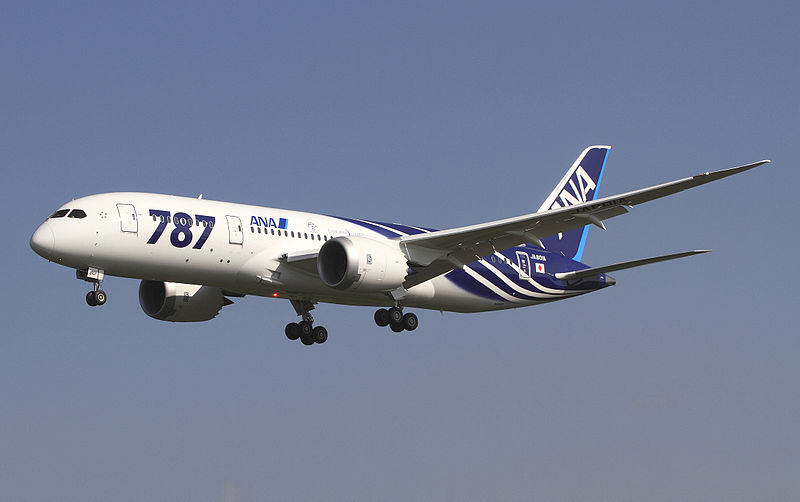
\includegraphics[width=\textwidth]{images/800px-All_Nippon_Airways_Boeing_787-8_Dreamliner_JA801A_OKJ_in_flight.jpg}\\\hfill (credit Spaceaero2, wikipedia)}
\only<2>{\begin{center}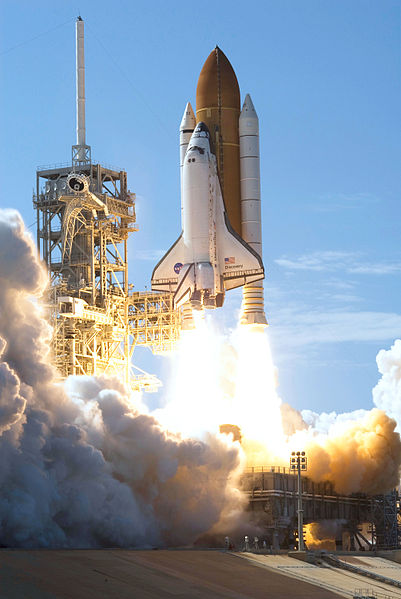
\includegraphics[width=.8\textwidth]{images/401px-STS-124_launch_from_a_distance.jpg}\end{center}}
\only<3>{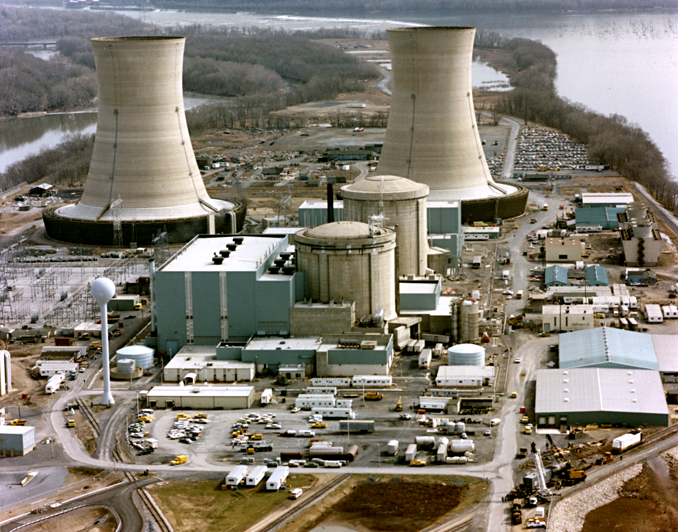
\includegraphics[width=\textwidth]{images/Three_Mile_Island_(color)-2.jpg}}
\only<4>{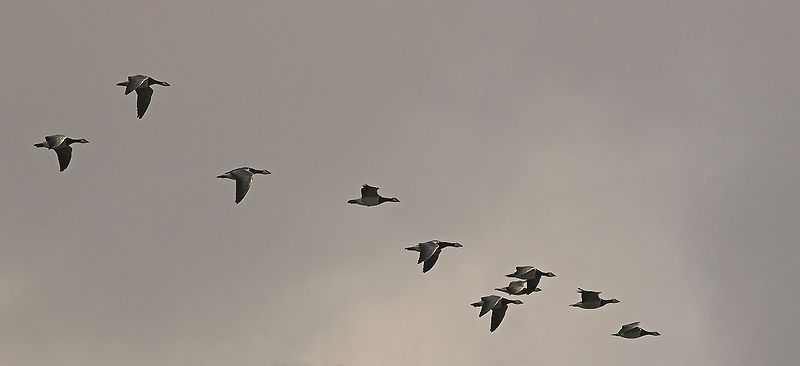
\includegraphics[width=\textwidth]{images/800px-BrantaLeucopsisMigration.jpg}\\ \hfill (credit Thermos, wikipedia)}
\only<5>{\begin{center}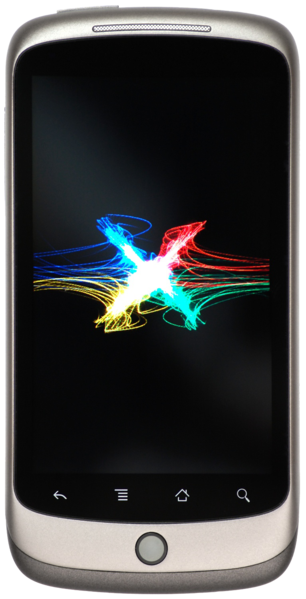
\includegraphics[width=.3\textwidth]{images/306px-Nexus_One.png}\end{center}}

\end{frame}


\begin{frame}
\frametitle{Models are Inherently Wrong}
\begin{changemargin}{1cm}

\begin{quote}
\textit{...essentially, all models are wrong, but some are useful.}
\end{quote}
\hfill George E. P. Box

\end{changemargin}
\end{frame}

\begin{frame}
\frametitle{Models are Inherently Wrong}
\begin{changemargin}{1cm}

Simulation is an abstraction and not as detailed as reality.

$\pi$ has an infinite number of digits. After the first thousand digits, the error introduced by rounding is so small it has no relevance for architectural calculations. 

How much is ``enough'' is a matter of engineering judgement.

\end{changemargin}
\end{frame}

\begin{frame}
\frametitle{Model Validity}
\begin{changemargin}{1cm}
Critical element: models have a range of validity.

This range must be respected if the model is useful.

Outside the range, the model is useless or misleading.

\end{changemargin}
\end{frame}


\begin{frame}
\frametitle{Model Validity Example: Physics}
\begin{changemargin}{1cm}
Newton's equations are valid at speeds below 0.1$c$.\\
\quad \small{Where $c$ is the speed of light in a vacuum.}

In that range, the error is small and can be ignored.

If you try to apply it at speeds of 0.5$c$, your answer is wrong.

Instead, use Einstein's equations as the model.\\
\quad They have a different (larger) range of validity.

Key point: understand the model's limitations.

\end{changemargin}
\end{frame}

\begin{frame}
\frametitle{The Map and the Territory}
\begin{changemargin}{1cm}

\begin{quote}
\textit{The map is not the territory.}
\end{quote}
\hfill Alfred Korzybski

\end{changemargin}
\end{frame}

\begin{frame}
\frametitle{The Map and the Territory}
\begin{changemargin}{1cm}
Don't confuse the map (abstraction) and territory (reality).

The model can be helpful, but don't overdo it.

Don't spend all your time modelling or studying model output.

Also take time to understand the real challenges.

\end{changemargin}
\end{frame}

\begin{frame}
\frametitle{The Map and the Territory: Example}
\begin{changemargin}{1cm}
A literal example of the map and territory: Canada-US Border.

West of Ontario, the border drawn on most maps as being exactly the $49^{th}$ parallel.

This is, however, wrong.

\end{changemargin}
\end{frame}

\begin{frame}
\frametitle{The Map and the Territory: Example}
\begin{changemargin}{1cm}
Surveyors placed small monuments at discrete distances.

The border is legally the series of line segments connecting these monuments.

Given the level of technology available at the time of measurement, these are not in a perfectly straight line.

\end{changemargin}
\end{frame}

\begin{frame}
\frametitle{The Map and the Territory: Example}
\begin{changemargin}{1cm}
Even a map representing those is wrong.

Shrinking thousands of kilometres of country down to centimetres will introduce error and inaccuracy.

How small can you print the dots marking the monuments?

\end{changemargin}
\end{frame}


\begin{frame}
\frametitle{Case studies}

\begin{center}
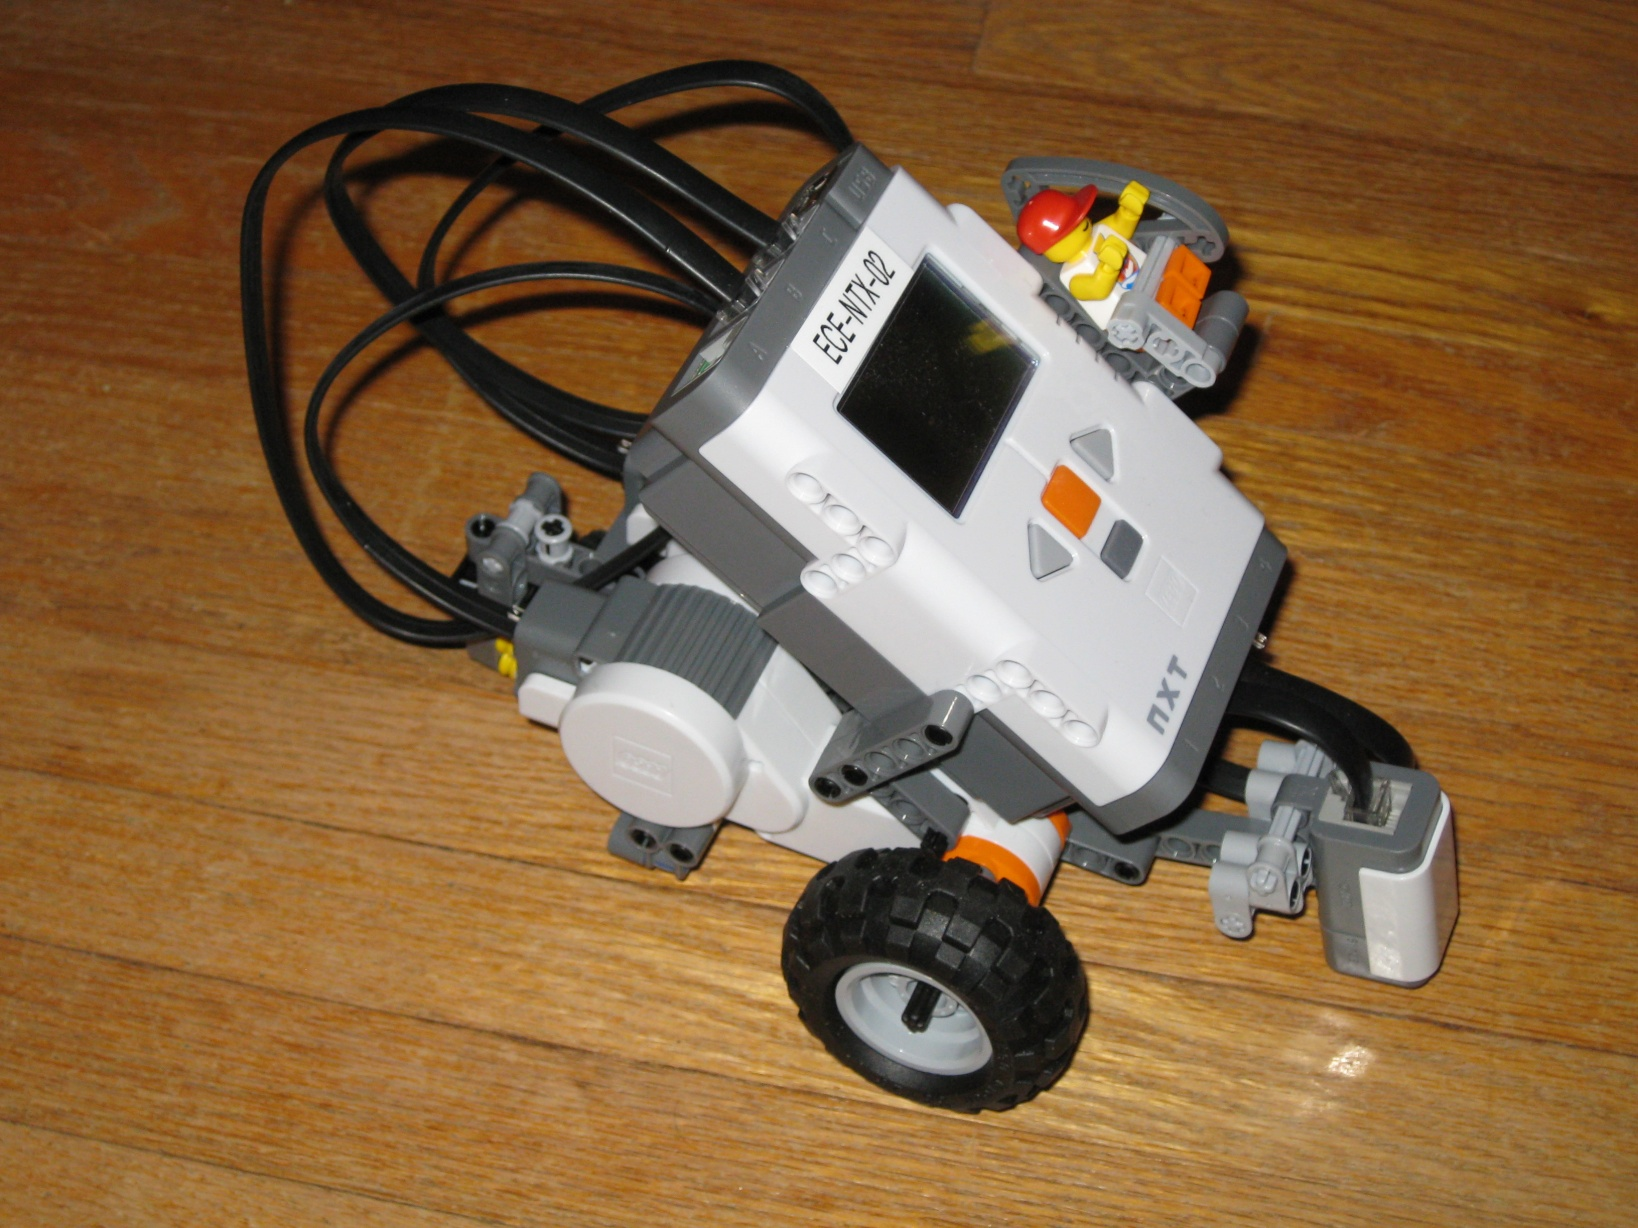
\includegraphics[width=.9\textwidth]{images/tribot}
\end{center}

\end{frame}

\begin{frame}
\frametitle{Coarse Simulation}

\begin{changemargin}{1cm}
\Large
Create a set of classes:

\begin{itemize}
\only<1>{\item class Board: says whether the class is black or white at
a point.

\begin{center}
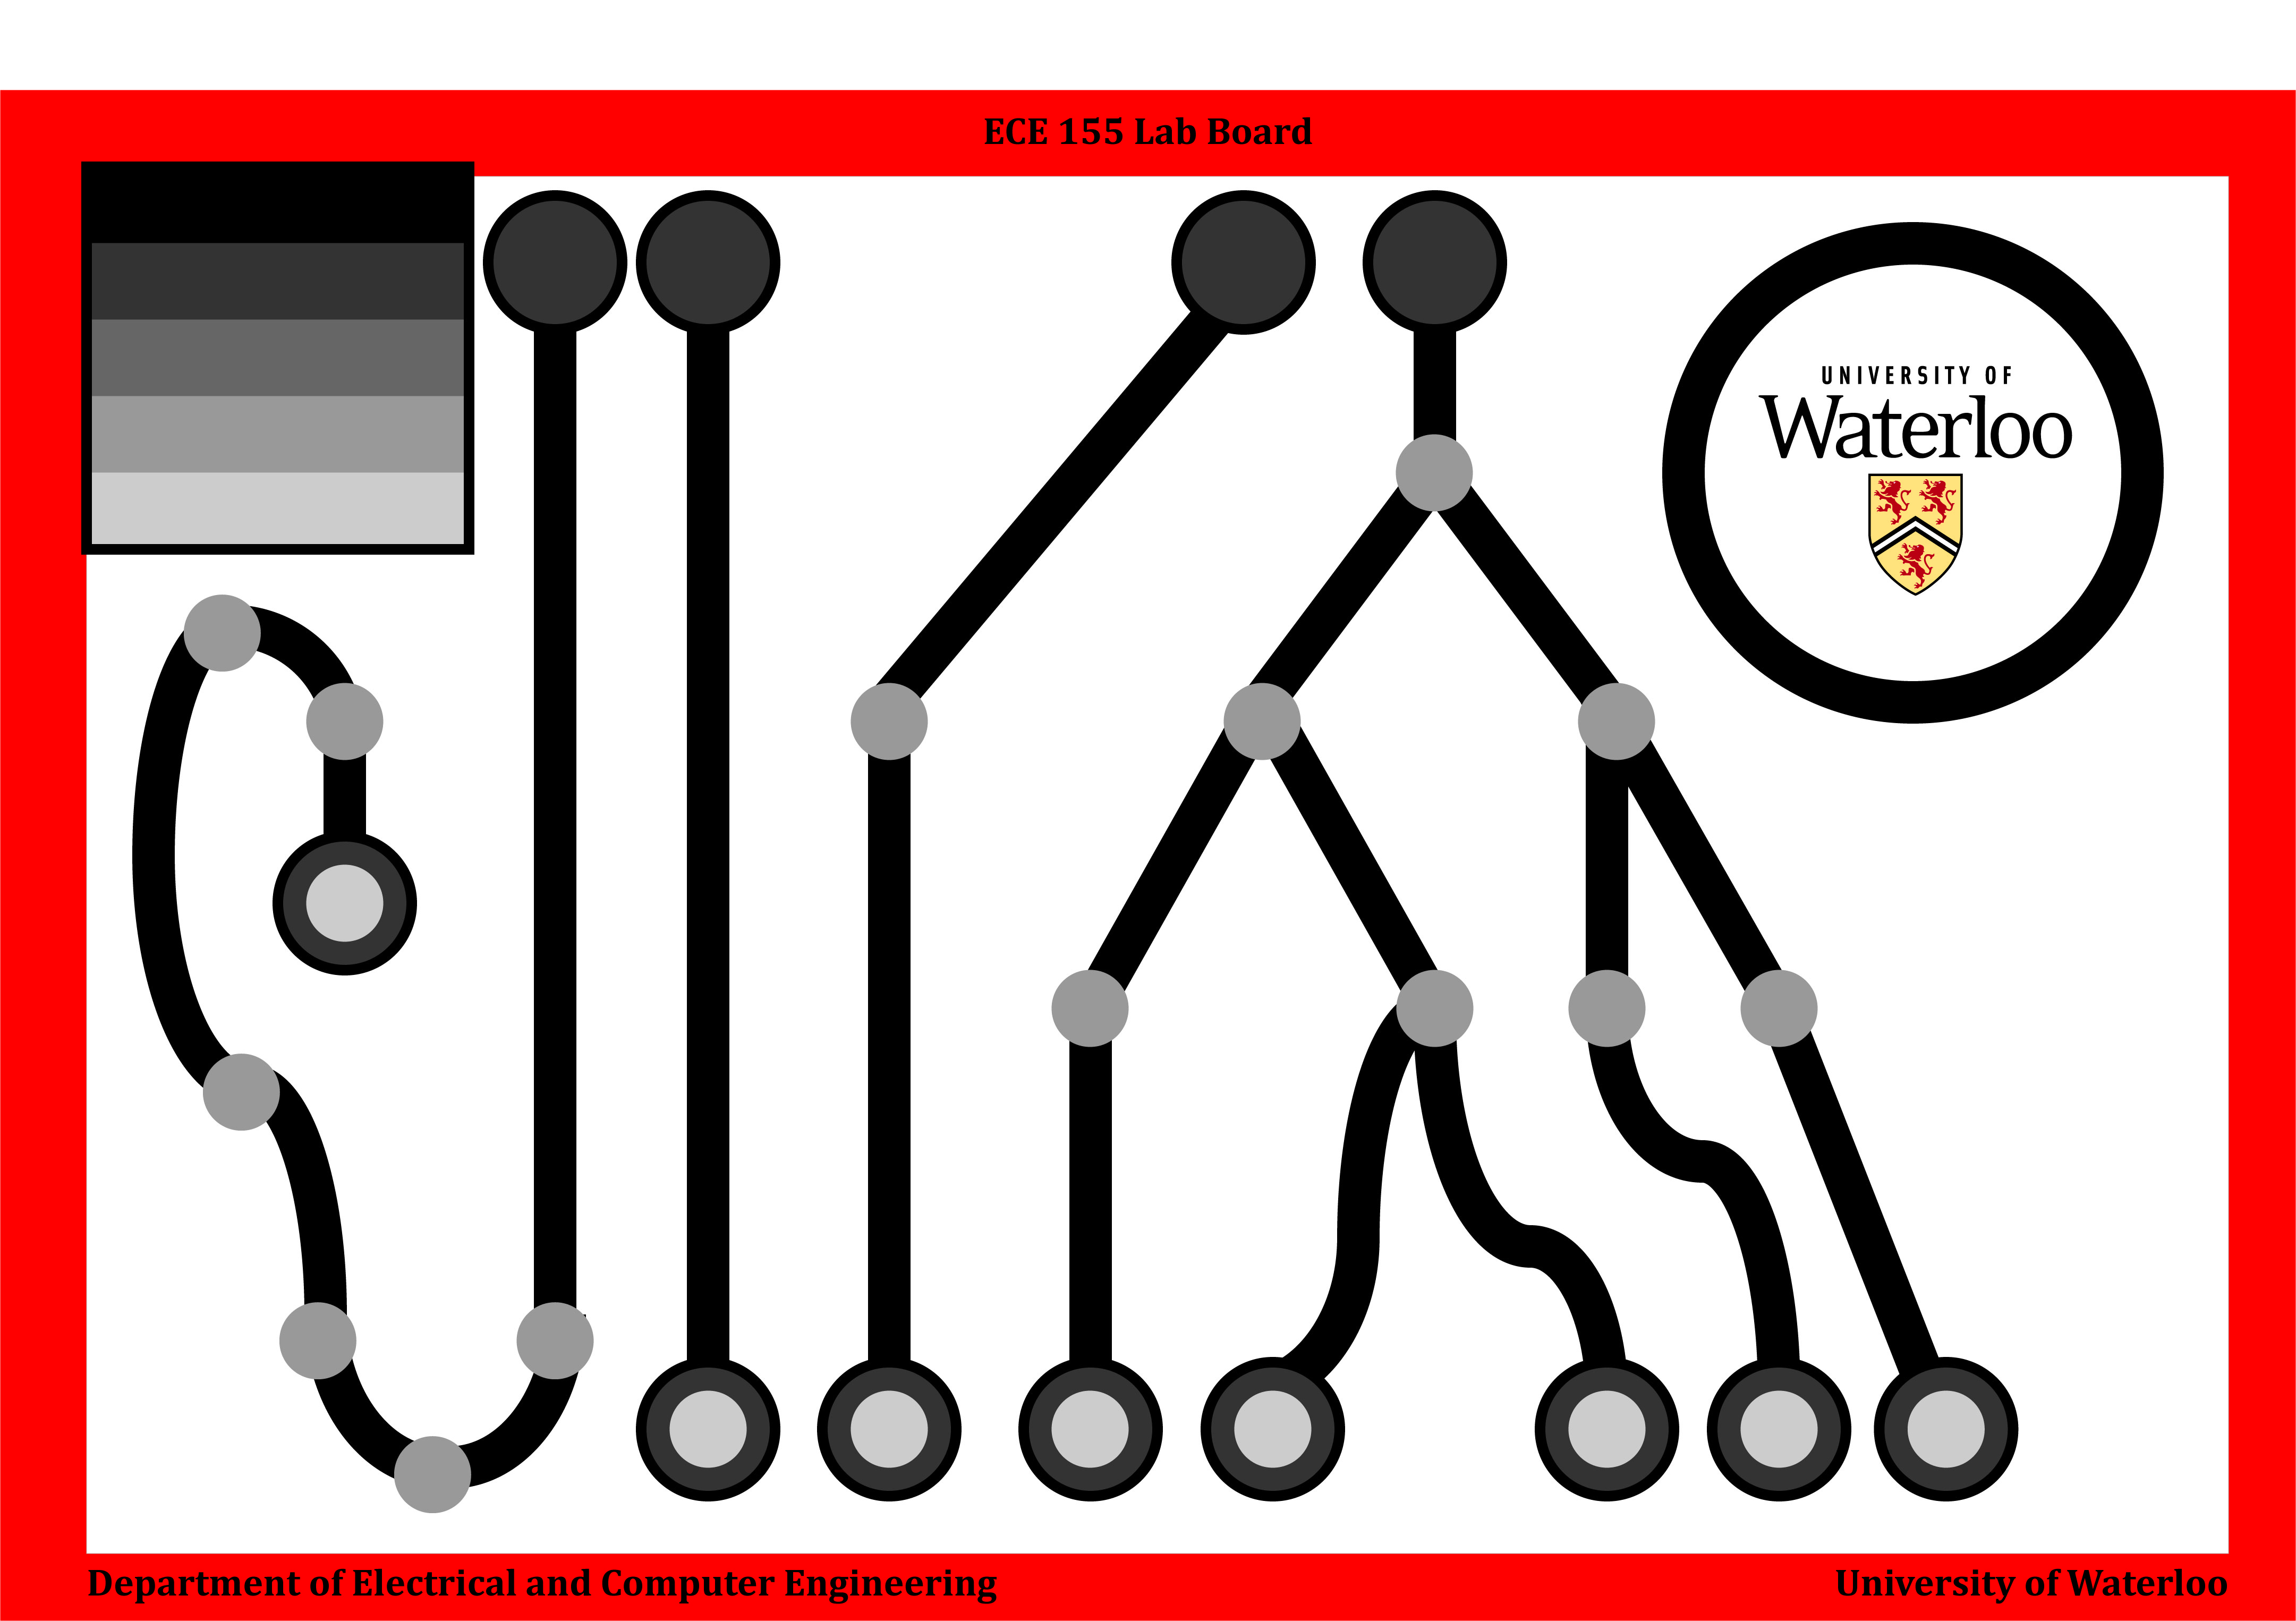
\includegraphics[width=.5\textwidth]{images/lab-board}
\end{center}
}
\only<2>{\item class Robot: simulates the position and velocity of the robot;
contains main logic.

\begin{center}
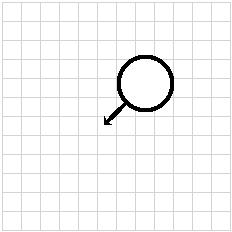
\includegraphics[width=.4\textwidth]{images/coarse-sim}
\end{center}
}

\only<3>{
\item class LightSensor: provides an interface between the
{\tt Robot} and the {\tt Board}.
}
\end{itemize}

\end{changemargin}

\end{frame}

\begin{frame}
\frametitle{Coding the Coarse Simulation}

\begin{changemargin}{2.5cm}

\Large
You'd provide a main simulation driver, which calls the {\tt Robot} to:
\begin{itemize}
\item update its position according to its velocity;
\item turn the robot if necessary.
\end{itemize}
~\\

Each call to the {\tt Robot}'s update simulates the effect of time moving forward
by one time-step.

\end{changemargin}

\end{frame}

\begin{frame}

\frametitle{\small Detailed Simulation: Visual Simulation Environment}

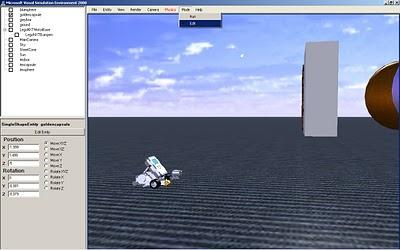
\includegraphics[width=\textwidth]{images/vse-shot1}
\begin{changemargin}{2.5cm}
Implements physics. Calls your actual code.
\end{changemargin}
\end{frame}

\begin{frame}

\frametitle{Simulation Caveat}

\begin{changemargin}{2.5cm}
\huge
Paraphrased: ``Everything worked fine in simulation, but needed
lots more work in reality.''
\end{changemargin}

\end{frame}

\begin{frame}
\frametitle{Other Simulation Examples}
\begin{center}
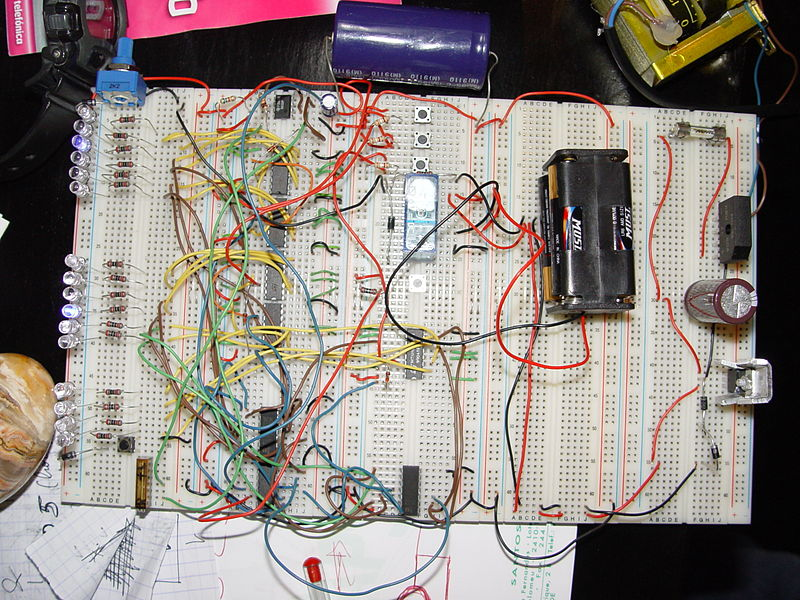
\includegraphics[width=.7\textwidth]{images/800px-Relogio_binario}
\end{center}

\begin{changemargin}{1cm}
Use discrete techniques: gates change values at specific times,
in response to changing inputs.
\end{changemargin}
\end{frame}

\begin{frame}
\frametitle{Other Simulation Examples}
\begin{center}
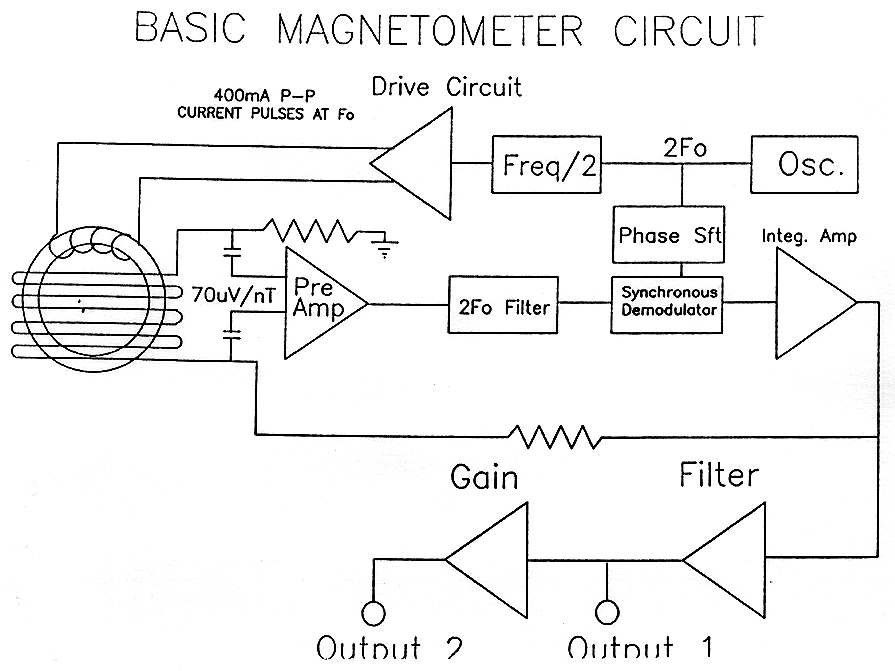
\includegraphics[width=.7\textwidth]{images/fig6}

\hfill (credit: Russell et al, \url{http://www-ssc.igpp.ucla.edu/personnel/russell/papers/ggs-polar/})
\end{center}

\begin{changemargin}{1cm}
Analog circuit: continuous techniques.
\end{changemargin}
\end{frame}

\begin{frame}
\frametitle{Techniques for simulation}

\Large
\begin{changemargin}{1cm}
\begin{itemize}
\item Discrete: use an event queue.
\item Continuous: numerically integrate an ordinary differential equation repeatedly (ECE204).
\end{itemize}
\end{changemargin}
\end{frame}

\begin{frame}
\frametitle{Classifying simulations: Three axes}

\begin{center}
\tdplotsetmaincoords{60}{125}
\begin{tikzpicture}
		[tdplot_main_coords,
			cube/.style={very thick,black},
			grid/.style={very thin,gray},
			axis/.style={->,blue,thick}]

	%draw the axes
	\draw[axis] (0,0,0) -- (3,0,0) node[anchor=east]{continuous/discrete};
	\draw[axis] (0,0,0) -- (0,3,0) node[anchor=west]{dynamic/static};
	\draw[axis] (0,0,0) -- (0,0,3) node[anchor=west]{deterministic/stochastic};
	
\end{tikzpicture}
\end{center}

\end{frame}

\begin{frame}
\frametitle{Discrete versus Continuous}

\Large
\begin{changemargin}{1cm}
\begin{itemize}
\item Discrete: time steps ahead in increments (e.g. finite state machine)
\item Continuous: evaluate at discrete times, but system has values at all times.
\end{itemize}
\end{changemargin}
\end{frame}

\begin{frame}
\frametitle{Dynamic versus Static}

\Large
\begin{changemargin}{1cm}
\begin{itemize}
\item Dynamic: system evolves over time; recomputes state.
\item Static: one-shot deal \\(e.g. what-if simulations).
\end{itemize}
\end{changemargin}
\end{frame}


\begin{frame}
\frametitle{Deterministic versus Stochastic}

\begin{changemargin}{1cm}
\begin{itemize}
\item Deterministic: exactly computes state at every step
\item Stochastic: uses randomness to guess expected behaviour (with high accuracy).
\end{itemize}
\end{changemargin}
\end{frame}

\begin{frame}
\frametitle{Simulation Tools}

\begin{changemargin}{1cm}
Some examples:
\begin{itemize}
\item \emph{Microsoft Visual Simulation Environment}: MS robotics.
\item \emph{Arena}: businesses, services, and manufacturing processes.
\item \emph{Simulink}: time-varying systems, e.g. communications, controls, signal processing, video processing, and image processing.
\item \emph{SPICE} \& variants: analog circuits.
\end{itemize}

Also: simulator-building languages.
\end{changemargin}

\end{frame}

\end{document}
